%
% skalar.tex -- Skalarprodukt
%
% (c) 2018 Prof Dr Andreas Müller, Hochschule Rapperswil
%
\section{Orthogonale Projektion und Skalarprodukt\label{section:ortho-skalar}}
\rhead{Orthogonale Projektion und Skalarprodukt}
\index{Skalarprodukt}
Abstand und Winkel spielen in der euklidischen Geometrie eine fundamentale
Rolle, die bisher eingeführten Elemente der Vektorgeometrie erlauben
jedoch noch nicht, Abstände oder Winkel zu berechnen.
Aus der elementaren Trigonometrie ist bekannt, dass der Schlüssel dazu
das Verständnis rechtwinkliger Dreiecke ist.
Der Kosinus eines Winkels ist das Verhältnis von Ankathete zu Hypothenuse.
De Ankathete ist aber auch die orthogonale Projektion der Hypothenuse
auf die Richtung der Ankathete.
Das Skalarprodukt soll daher aus der orthogonalen Projektion entwickelt
werden.

%
% Orthgonale Projektion
%
\subsection{Orthogonale Projektion\label{subsection:orthoproj}}
\index{orthogonale Projektion}
\index{Projektion!orthogonale|see{orthogonale Projektion}}
Zunächst möchten wir zeigen, dass sich Längen und Winkel berechnen
lassen, wenn man in der Lage ist, die Länge der orthogonalen Projektion
eines Vektors $\vec{v}$ auf jeden beliebigen anderen Vektor $\vec{u}$
zu berechnen.
\begin{figure}
\begin{center}
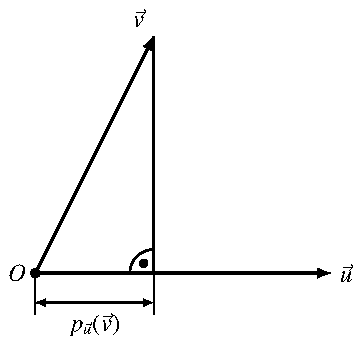
\includegraphics{4/images/projektion.pdf}
\end{center}
\caption{Orthogonale Projektion\label{orthproj}}
\end{figure}

Seien also $\vec u$, $\vec v$ zwei beliebige Vektoren wie in Abbildung~\ref{orthproj}, und $p_{\vec u}(\vec v)$
die Länge der Projektion des Vektors $\vec v$ auf $\vec u$.
Wir versehen diese Länge mit einem Vorzeichen, zeigt der auf $\vec u$
projizierte Vektor $\vec v$ in die gleiche Richtung wie $\vec u$
nehmen wir die Länge positiv, zeigt der projizierte Vektor in die
Gegenrichtung, ist $p_{\vec u}(\vec v)$ negativ.

Die Länge von $\vec v$ ist $p_{\vec v}(\vec v)$, und für den Winkel
$\alpha$ zwischen den beiden Vektoren ist
\begin{equation}
\cos \alpha = \frac{p_{\vec u}(\vec v)}{p_{\vec v}{\vec v}}.
\label{zwischenwinkel}
\end{equation}
Offenbar ist die Länge der Projektion die grundlegendere Grösse,
aus der man die anderen Konzepte ableiten kann.
Etwas ungünstig ist an dieser Projektion nur, dass die beiden Vektoren nicht
symmetrisch eingehen.
\begin{figure}
\centering
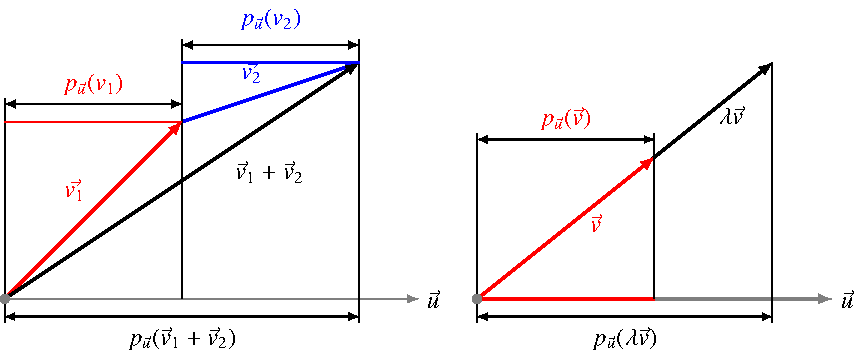
\includegraphics{4/images/linearitaet.pdf}
\caption{Die Projektionsabbilung
$\vec{v}\mapsto p_{\vec{u}}(\vec{v})$
ist linear. Die linke Graphik zeigt
$p_{\vec{u}}(\vec{v}_1+\vec{v}_2)
=
p_{\vec{u}}(\vec{v}_1)+p_{\vec{u}}(\vec{v}_2)$,
die rechte ist der Strahlensatz und zeigt
$p_{\vec{u}}(\lambda\vec{v})=\lambda p_{\vec{u}}(\vec{v})$.
\label{projektionlinearitaet}}
\end{figure}
Immerhin ist $p_{\vec u}(\vec v)$ linear in $\vec v$, wie man
sich mit der Abbildung~\ref{projektionlinearitaet}
sofort überzeugen kann, es ist also
\begin{align*}
p_{\vec u}(\vec v_1+\vec v_2)&=p_{\vec u}(\vec v_1)+p_{\vec u}(\vec v_2)\\
p_{\vec u}(\lambda \vec v)&=\lambda p_{\vec u}(\vec v).
\end{align*}

%
% Skalarprodukt
%
\subsection{Skalarprodukt}
\index{Skalarprodukt}
\begin{figure}
\begin{center}
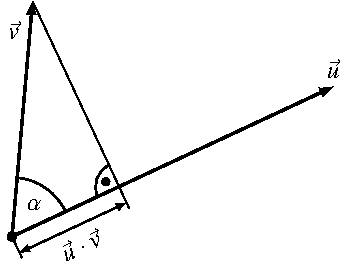
\includegraphics{4/images/skalarprodukt.pdf}
\end{center}
\caption{Skalarprodukt $\vec u\cdot \vec v$ des Einheitsvektors $\vec u$
und des Vektors $\vec v$ mit Zwischenwinkel
$\alpha$.\label{image-skalarprodukt}}
\end{figure}
Gesucht ist daher eine Konstruktion, welche immer noch linear ist,
aber auch symmetrisch in $\vec u$ und $\vec v$.
Die Formel (\ref{zwischenwinkel}) deutet auch an, wie dies erreicht
werden kann.
Der Zwischenwinkel kann natürlich auch berechnet werden,
indem die beiden Vektoren vertauscht werden:
\[
\cos \alpha
=
\frac{p_{\vec u}(\vec v)}{p_{\vec v}(\vec v)}
=
\frac{p_{\vec v}(\vec u)}{p_{\vec u}(\vec u)}
\]
Multipliziert man diese Gleichung mit
$
p_{\vec u}(\vec u)
p_{\vec v}(\vec v)
$, erhält man
\[
\vec u\cdot\vec v
=
p_{\vec u}(\vec u)
p_{\vec v}(\vec v)
\cos\alpha =
p_{\vec u}(\vec u)p_{\vec u}(\vec v)
=
p_{\vec v}(\vec v)p_{\vec v}(\vec u),
\]
was offenbar symmetrisch in $\vec u$ und $\vec v$ ist.

\begin{definition}Das Skalarprodukt zweier Vektoren $\vec u$ und
$\vec v$ ist
\[
\vec u\cdot\vec v
=
p_{\vec u}(\vec u)
p_{\vec v}(\vec v)
\cos\alpha.
\]
\end{definition}
Diese Grösse ist linear in $\vec u$ und linear in $\vec v$, und man kann
daraus $p_{\vec u}(\vec v)$ mittels
\[
p_{\vec u}(\vec v)
=
\frac{p_{\vec u}(\vec v)p_{\vec u}(\vec u)}{p_{\vec u}(\vec u)}
=
\frac{\vec u\cdot\vec v}{\sqrt{p_{\vec u}(\vec u)^2}}
=
\frac{\vec u\cdot\vec v}{\sqrt{\vec u\cdot \vec u}}
\]
wieder zurückgewinnen.

\begin{satz}
Seien $\vec u$ und $\vec v$ zwei Vektoren, dann ist
\[
|\vec u|=p_{\vec u}(\vec u)=\sqrt{\vec u\cdot\vec u}
\]
die Länge des Vektors, und für den Zwischenwinkel $\alpha$ gilt
\[
|\vec u|\,|\vec v|\cos\alpha=\vec u\cdot\vec v
\]
Zwei vom Nullvektor verschiedene Vektoren  stehen genau dann senkrecht
aufeinander, wenn $\vec u\cdot\vec v=0$.
Die Projektion $\vec v_{\|}$ von $\vec v$ auf $\vec u$ ist
\[
\vec v_{\|}=\frac{\vec v\cdot\vec u}{\vec u\cdot\vec u}\vec u.
\]
Ist $\vec u$ ein Einheitsvektor, dann ist $\vec v_{\|}=(\vec v\cdot \vec u)\vec u$.
\end{satz}
\index{Zwischenwinkel}

%
% Skalarprodukt und Standardbasis
%
\subsection{Skalarprodukt und Standardbasis}
Zur praktischen Berechnung des Skalarproduktes benötigen wir
eine Formel, die das Skalarprodukt aus den Vektorkomponenten
berechnet.
Schreibt man
\[
\vec u=\begin{pmatrix}u_1\\u_2\\u_3\end{pmatrix}
=u_1\vec e_1+u_2\vec e_2+u_3\vec e_3
,
\qquad
\vec v=\begin{pmatrix}v_1\\v_2\\v_3\end{pmatrix}
=v_1\vec e_1+v_2\vec e_2+v_3\vec e_3
\]
dann kann das Skalarprodukt mit der Linearität berechnet werden:
\begin{align*}
\vec u\cdot\vec v
&=
(u_1\vec e_1+u_2\vec e_2+u_3\vec e_3)\cdot
(v_1\vec e_1+v_2\vec e_2+v_3\vec e_3)
\\
&=
u_1v_1\vec e_1\cdot\vec e_1+
u_1v_2\vec e_1\cdot\vec e_2+
u_1v_3\vec e_1\cdot\vec e_3\\
&\qquad +
u_2v_1\vec e_2\cdot\vec e_1+
u_2v_2\vec e_2\cdot\vec e_2+
u_2v_3\vec e_2\cdot\vec e_3\\
&\qquad+
u_3v_1\vec e_3\cdot\vec e_1+
u_3v_2\vec e_3\cdot\vec e_2+
u_3v_3\vec e_3\cdot\vec e_3
\end{align*}
Die Skalarprodukte von aufeinander senkrecht stehenden Vektoren
verschwinden, es bleiben nur die Termen mit $\vec e_i\cdot\vec e_i$,
das Skalarprodukt eines Vektors mit sich selbst ist das Quadrat
der Länge, also $\vec e_i\cdot \vec e_i=1$ und so erhalten wir den
Satz
\begin{satz}
Das Skalarprodukt zweier Vektoren
\[
\vec u=\begin{pmatrix}u_1\\u_2\\u_3\end{pmatrix},
\qquad
\vec v=\begin{pmatrix}v_1\\v_2\\v_3\end{pmatrix}
\]
ist
\[
\vec u\cdot\vec v
=
u_1v_1+u_2v_2+u_3v_3.
\]
\end{satz}

\begin{beispiel}
Berechne die Länge und den Zwischenwinkel der Vektoren
\begin{align*}
\vec a&= \begin{pmatrix} 3\\12\\ 4 \end{pmatrix},
&
\vec b&= \begin{pmatrix}2\\3\\6\end{pmatrix}.
\end{align*}

\smallskip

{\parindent 0pt Die} Länge der Vektoren ist
\begin{align*}
|\vec a|
&
=\sqrt{\vec a\cdot \vec a}
&
|\vec b|
&
=\sqrt{\vec b\cdot \vec b}
\\
&=\sqrt{9+144+16}
&
&=\sqrt{4+9+36}
\\
&=\sqrt{169}=13
&
&
=\sqrt{49}=7
\end{align*}
Damit kann man jetzt auch den Zwischenwinkel berechnen
\begin{align*}
\cos\alpha&= \frac{\vec a\cdot \vec b}{|\vec a|\;|\vec b|}
=
\frac{6+36+24}{13\cdot 7}=\frac{66}{91}=0.72527
\\
\alpha&=43.51^\circ
\end{align*}
\end{beispiel}
Häufig braucht man zu einem Vektor einen Vektor mit gleicher Richtung,
aber Einheitslänge.
Wir verwenden die Schreibweise
\[
\vec{v}^0 = \frac{\vec{v}}{|\vec{v}|}
\]
für den zum Vektor $\vec{v}$ gehörigen Einheitsvektor.

